\documentclass[b5j,dvipdfmx]{jsarticle}

\usepackage{mystyle,tikz,wrapfig,eclbkbox}
\usetikzlibrary{intersections,calc}

\begin{document}

\section{数学1A}

\subsection{数と式}

\subsubsection{集合と命題}

まず数学で扱ういわゆる問題について次のように定めておく.

\begin{definition}
正しいか正しくないかを決めることができる文を{\bf 命題}という. また, 命題が正しいときその命題は{\bf 真}であるといい, 正しくないときその命題は{\bf 偽}であるという.
\end{definition}

次の例で見るように, 命題を書くとき, 誤解の無いよう「」または『』で囲うことがあるが, これは省略してもよい. また, 命題そのものを文字で置くことがあるが, そのときは大抵$p$, $q$, $r, \ldots$のように$p$から順番に用いて表す\footnote{propositionの頭文字である.}.

\begin{example}
「2は偶数である」は命題であり, 真である. また, 「2は奇数である」は命題であり, 偽である. 「2は美しい」は人によって真偽が変わるから, 命題でない.
\end{example} 

\begin{example}
「水は液体である」は命題であり, 真である. 「水は水である」は命題であり, 真である. 
\end{example}

\begin{example}\label{ex:prop}
「$x-1=3$」は$x$が何か分からないので真偽を判定できないから, 命題でない(「$x-1$は3である」と読み替えると分かりやすい). しかし, $x$に4を代入すれば「$3=3$」という真の命題となり, $x$に3を代入すれば「$2=3$」という偽の命題となる.
\end{example}

例\ref{ex:prop}のような, $x$を定めることで命題となる文を{\bf $x$に関する条件}, または単に{\bf 条件}という. 

\begin{definition}
$p$, $q$は条件とする.
\begin{enumerate}
	\item 「$p$であり$q$である」という条件を「$p$かつ$q$」で表す.
	\item 「$p$が真または$q$が真」という条件を「$p$または$q$」で表す. \label{def:logic_lor}
	\item 「$p$でない」という条件を$p$の{\bf 否定}といい, $\overline p$で表す.
	\item 「$p$が真のとき$q$も真である」という条件を「$p$ならば$q$」または$p\Rightarrow q$で表す. また, $p\Rightarrow q$が真のとき, $p$は$q$であるための{\bf 十分条件}であるといい, $q$は$p$であるための{\bf 必要条件}であるという. \label{def:logic_implication}
	\item 『「$p\Rightarrow q$」かつ「$q\Rightarrow p$」』という命題を$p\Leftrightarrow q$で表す. $p\Leftrightarrow q$が真のとき, $p$は$q$であるための{\bf 必要十分条件}である, または$p$と$q$は{\bf 同値}であるという.
\end{enumerate}
\end{definition}

\begin{example}

\end{example}

与えられた条件を真にするような$x$を, ある程度分かりやすく考えるために, 集合という概念を学ぶ.

\begin{definition}
ある条件を満たすものの集まりを{\bf 集合}といい, 集合を構成するものそれぞれを{\bf 要素}または{\bf 元}という. また, $x$が集合$X$の要素の1つであるとき, $x$は$X$に{\bf 属する}といい, $x\in X$と表す. 
\end{definition}

大抵の場合, 集合は$A$, $B$などの大文字, 要素は$a$, $b$などの小文字を用いて表す. また, $x$が集合$X$に属さないことを$x\notin X$で表す. さらに, 左右を入れ替えて$X\ni x$や$X\not\ni x$と表すこともあるが, 意味することはそれぞれ変わらない. 

\begin{example}
0以上3以下の自然数全体の集合$A$を考える. $A$の要素$a$が満たす条件は「$a$は自然数かつ$0\leqq a\leqq 3$」である. 従って, $A$の要素は1, 2, 3の3つであり, $2\in A$や$4\notin A$などが成り立つ.

このとき, $A$の要素を明らかにして$A=\{1,2,3\}$と表すことができる. この表し方を外延的記法といい, 集合に属する要素が少ないときに有効である.
\end{example}

\begin{example}
集合$B=\{1,3,7\}$を考える. $B$の要素は明らかであるが, 定義に従うと, $B$の要素$b$が満たす条件は「$b=1$または$b=3$または$b=7$」である. 
\end{example}

\begin{example}\label{ex:set}
自然数全体の集合$N$を考える. $N$の要素$n$が満たすべき条件は「$n$は自然数である」である. 従って, $N$の要素は1, 2, 3, 4,$\ldots$のように無限に存在する. 

このとき, $N$の要素の満たす条件を用いて$N=\set{n}{n\text{は自然数}}$のように表すことができる. この表し方を内包的記法といい, 要素の条件が分かっているときに有効である.
\end{example}

\begin{definition}
要素を持たない集合を{\bf 空集合}といい, $\emptyset$で表す. 
\end{definition}

\begin{definition}
$A$, $B$を集合とする. すべての$A$の要素が$B$にも属しているとき, $A$は$B$の{\bf 部分集合}であるといい, $A\subset B$で表す. 
\end{definition}



\begin{definition}

\end{definition}

\subsection{必要性と十分性}

\section{数学2B}

\subsection{面積を求める積分}

2つの多項式に囲まれた面積を求めるとき, その立式が簡単にできる場合がある. 

$f(x)$, $g(x)$を多項式とする. 



\subsection{積分と平行移動}

置換積分

\subsection{二次関数と接線について}

\begin{wrapfigure}{l}{0.4\textwidth}
\centering
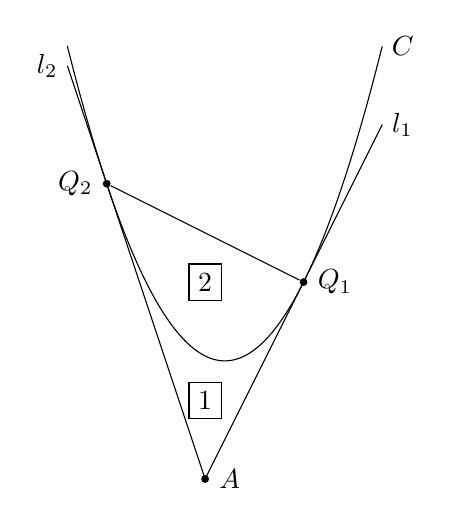
\begin{tikzpicture}
	\draw[samples=100,domain=-2:2] plot(\x,{pow(\x,2)}) node [right] {$C$};
	\draw[domain=-1/4:2] plot(\x,2*\x-1) node [right] {$l_1$};
	\draw[domain=-1/4:-2] plot(\x,-3*\x-9/4) node [left] {$l_2$};
	\node (Q1) at (-3/2,9/4) [inner sep=1pt,circle,fill=black,label=left:$Q_2$] {};
	\node (Q2) at (1,1) [inner sep=1pt,circle,fill=black,label=right:$Q_1$] {};
	\node (A) at (-1/4,-3/2) [inner sep=1pt,circle,fill=black,label=right:$A$] {};
	\draw (Q1)--(Q2);
	\node at (-1/4,1) [draw] {$2$};
	\node at (-1/4,-1/2) [draw] {$1$};
\end{tikzpicture}
\caption{}\label{pic:2_int_quadratic_function}
\end{wrapfigure}

二次関数$y=ax^2+bx+c\ (a\ne0)$のグラフ$C$に, ある点$A$から2本の接線$l_1$, $l_2$を引けたとする. $C$と$l_1$の交点を$Q_1$, $C$と$l_2$の交点を$Q_2$とすれば, $C$は三角形$\triangle AQ_1Q_2$を分割し, その面積比は図\ref{pic:2_int_quadratic_function}のように$1:2$となる. 

\begin{proof}
$\triangle AQ_1Q_2$は平行移動によって面積を変えないから, $A=O=(0,0)$としても一般性を失わない. $A$から$C$に引いた接線の傾きを$m$, 接点を$P=(p,q)$とすれば, 条件より
\begin{numcases}{}
q=mp \label{eq:2.1.1}\\
q=ap^2+bp+c \label{eq:2.1.2}\\
m=2ap+b \label{eq:2.1.3}
\end{numcases}
を得る. (\ref{eq:2.1.1})に(\ref{eq:2.1.3})を代入して$q=2ap^2+bp$が分かり, さらにこれを(\ref{eq:2.1.2})に代入すれば, $p$についての2次方程式$ap^2-c=0$を得る. 仮定より, 相異なる接点が2つ存在するのだから, この2次方程式は異なる2つの実数解
\[
p=\pm\sqrt\frac ca
\]
をもつ. 簡単のために, 以下$p=\sqrt{c/a}$とする. このとき, $C$と直線$Q_1Q_2$に囲まれた面積を$S$, $C$と$l_1$, $l_2$に囲まれた面積を$T$とすれば, それぞれ
\begin{align*}
S&=\left|a\int_{-p}^p\left(x^2-p^2\right)\,dx\right|\\
&=\frac{4|a|}3p^3,
\end{align*}
\begin{align*}
T&=\left|a\int_{-p}^0\left(x+p\right)^2\,dx\right|+\left|a\int_0^p\left(x-p\right)^2\,dx\right|\\
&=\frac {2|a|}3p^3
\end{align*}
となるので, たしかに$S:T=2:1$となることが分かる.
\end{proof}

上では$A$を定めてから$l_1$, $l_2$を定めているが, この順番は逆でもよい. つまり, $C$に相異なる2つの接線$l_1$, $l_2$を引き, これらの接線の唯一の交点を$A$と定めてもよい. 一般に, 互いに平行でない2つの直線の交点はただ一つに定まる.

\section{発展的な内容}

\subsection{ほげ}


\begin{thebibliography}{9}
	\bibitem{kada}嘉田勝, 『論理と数学から始める数学の基礎』, 日本評論社, 2018
\end{thebibliography}
\end{document}